\section{Three-dimensional disks with beta cooling}\label{3ddisk}
We confirm the above results in 3D disks with vertical
structure. Accounting for the third dimension will weaken gravitational instabilities
because the disk mass is spread across some vertical extent. It is 
possible to incorporate this effect in the previous 2D framework, but doing so
introduces an additional `softening' parameter $H_\mathrm{sg}$ as discussed in
Appendix \ref{3dcorr}. It is more direct to solve the 3D eigenvalue
problem to avoid such uncertainties. Our numerical approach is
outlined in Appendix \ref{3d_method}. 

%We will find that while softening the
%self-gravity in 2D can produce qualitatively similar results to 3D, a
%quantitative match is  
%{\bf note: fast beta-cooling in 3D destablizes vertical modes (enables
%convection)}
%take k>0 wlog
%consider Gamma=1
%height s.t. rho(zmax) = 0.05 rho(0) avoid very low densities 

In the following examples we consider a vertically isothermal disk
($\Gamma=1$ in Eq. \ref{poly_vert}). Then in the viscous case $\alpha$ is vertically
constant (Eq. \ref{alpha_beta_relation}). We consider only even modes
about the mid-plane, and apply a numerical disk surface at $z=\zmax$
such that $\rho(\zmax)=0.05\rho_0$.     

%in practice eliminate density with poisson
\subsection{Inviscid 3D disk}

We consider a 3D inviscid disk with $\gamma=1.4$, $\qthree=0.71$, and $\theta=0$. 
The 3D gravity parameter $\qthree$ is defined by 
Eq. \ref{Q3d_def}. For such a disk, the corresponding Toomre parameter 
$Q=2Q_\mathrm{crit}$. Recall $Q_\mathrm{crit}$, defined by
Eq. \ref{qcrit_def}, is the Toomre parameter value such that the 2D
disk would be marginally stable in the absence of cooling. 

Fig. \ref{3d_inviscid} shows growth rates and the most unstable
wavenumbers obtained for this model. We also plot 2D
results with the 3D correction as described in Appendix
\ref{3dcorr}. The (empirically) chosen value of 
$H_\mathrm{sg}=0.64H$ results in a close match between 2D and 3D
growth rates, but the most unstable wavenumber in 3D is somewhat smaller. 
This offset reflects self-gravity being weakened in the vertical 
direction: a larger horizontal scale is required to achieve the same
strength of self-gravity as the 2D case. Similarly, 
choosing $H_\mathrm{sg}=0.53H$ matches the optimum wavenumbers, but
growth rates are over-estimated in 2D.    

\begin{figure}
  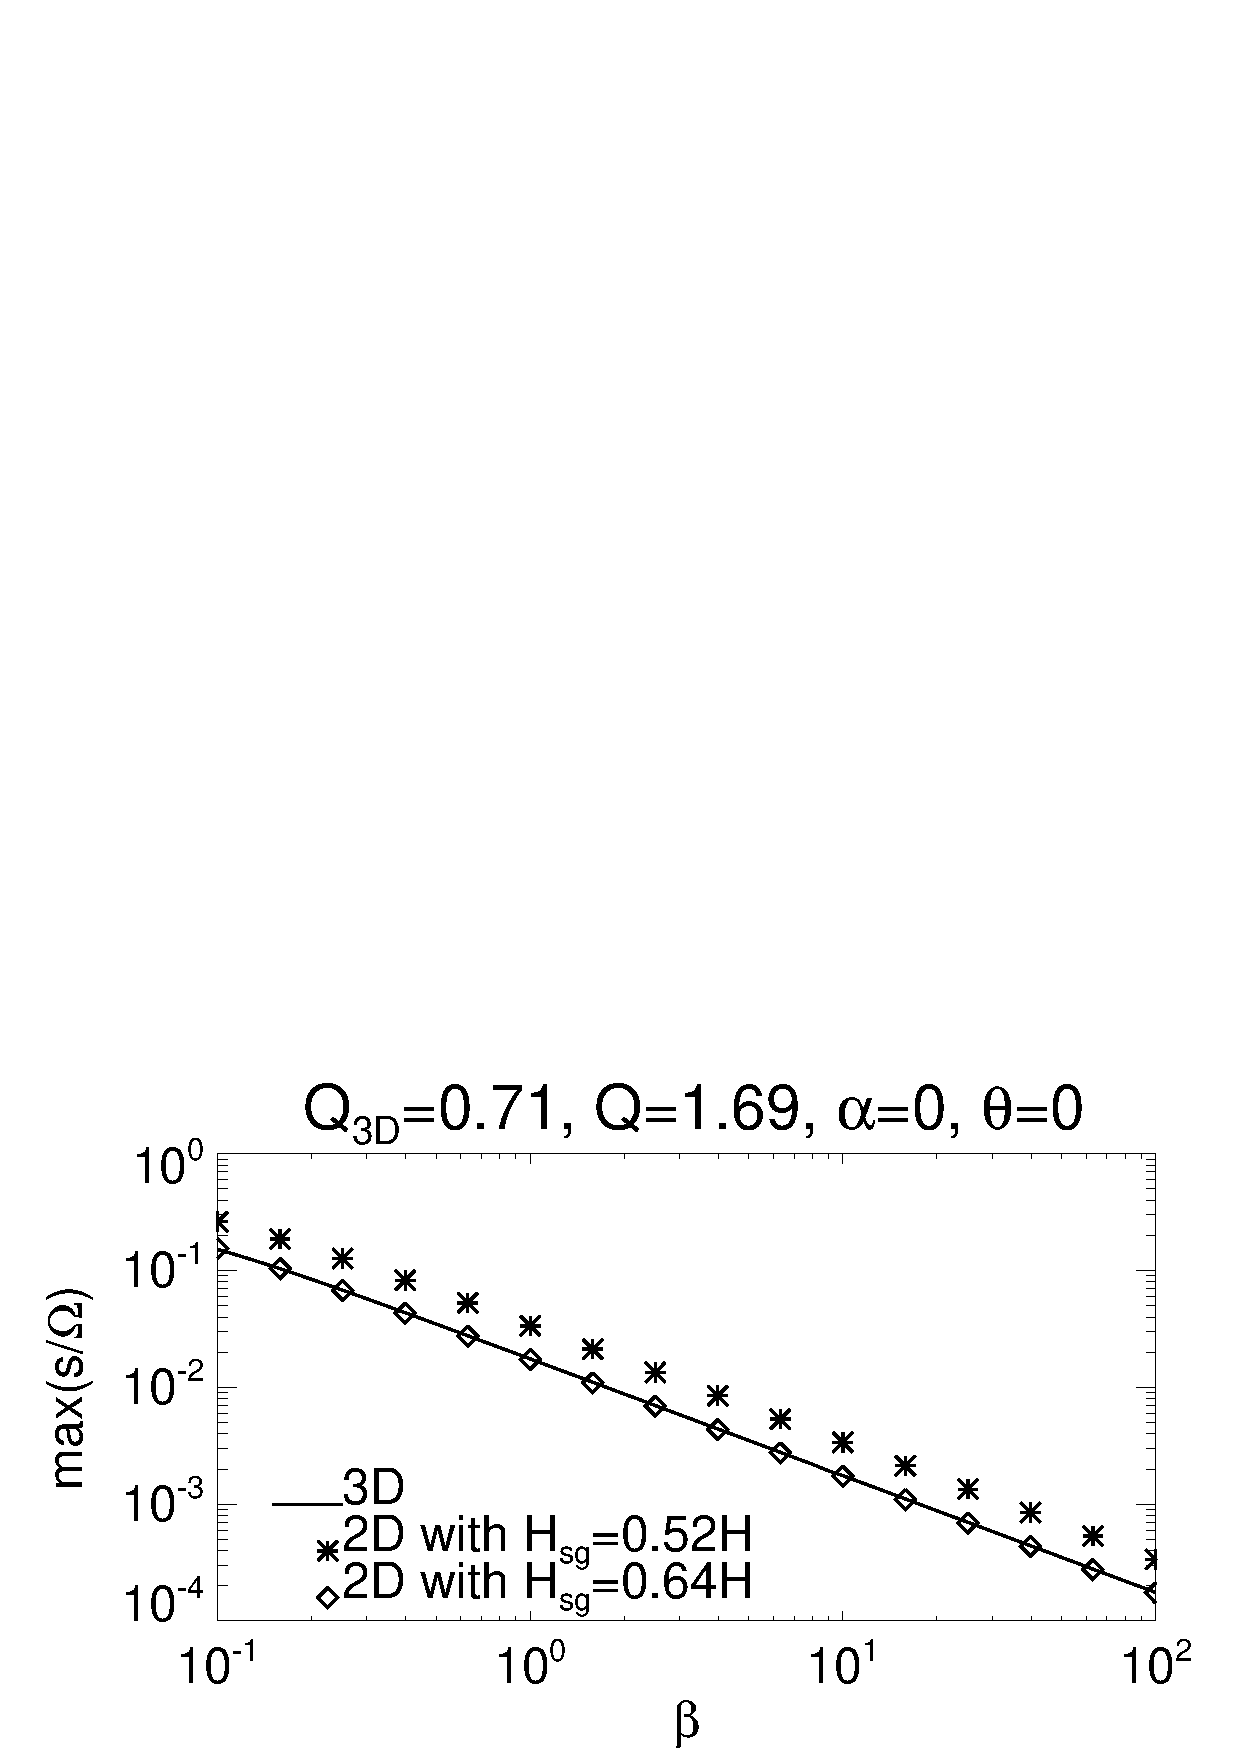
\includegraphics[width=\linewidth,clip=true,trim=0cm 2cm 0.cm
    0.0cm]{figures/3d_inviscid_rates}\\
  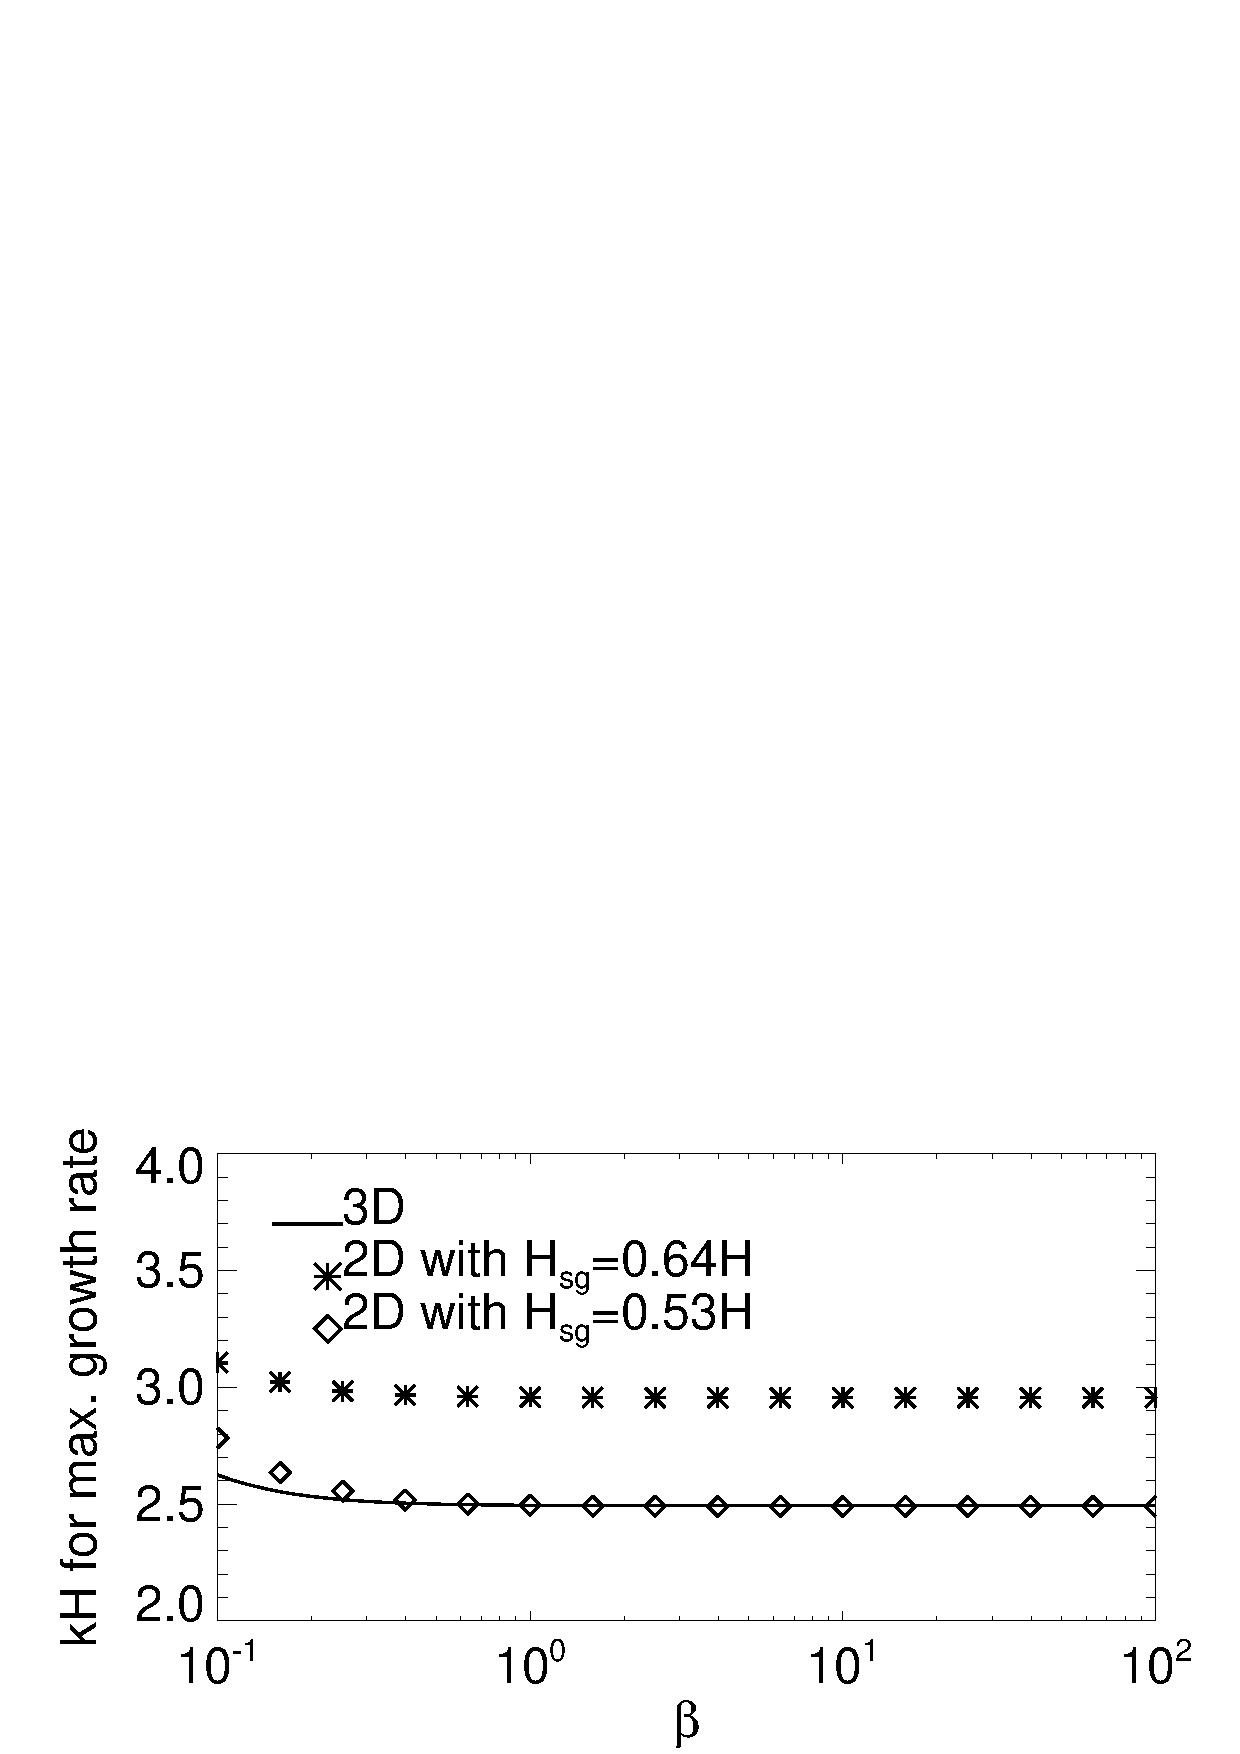
\includegraphics[width=\linewidth,clip=true,trim=0cm 0cm 0.cm
    0.8cm]{figures/3d_inviscid_kmax}
  \caption{Growth rates (top) and optimal wavenumber (bottom) obtained
    from the inviscid 3D eigenvalue problem (solid line). Asterisks
    and diamonds are corresponding values from the 2D dispersion
    relation (Eq. \ref{thindisk}) but with a softened gravity as
    described in Appendix \ref{3dcorr}. \label{3d_inviscid}} 
\end{figure}

\subsection{Viscous 3D disk} %growth rates, kmax, eigenfunction
For the 3D viscous problem we use the same set up as that in 2D
(\S\ref{2dvisc}), but with 
\begin{align}
  \qvert = \frac{Q_\mathrm{3D,crit}}{\sqrt{\alpha}}, \label{Q3d_visc_model}
\end{align}
where $Q_\mathrm{3D,crit}\simeq0.36$ is the 3D equivalent to the 2D
critical value, $Q_\mathrm{crit}$. Note that the background vertical
structure now varies with $\alpha$ through Eq. \ref{Q3d_visc_model},
which in turn depends on the cooling time through thermal
equilibrium (Eq. \ref{alpha_beta_relation}). 

Fig. \ref{3d_visc} shows growth rates, maximized over $k$, as a
function of the cooling time $\beta$. We also plot 2D results with 3D
corrections. Softening the self-gravity in 2D captures the correct 
qualitative behavior of the full 3D case. For $\beta\gtrsim 1$
choosing $H_\mathrm{sg}=0.8H$ produces a good match. However, it is
clear that a single, constant value of $H_\mathrm{sg}$ cannot
re-produce 3D growth rates for all $\beta$. This suggests that the
exact value of $H_\mathrm{sg}$ is problem-dependent, although taking 
$H_\mathrm{sg}\sim O(H)$ should give the correct 3D growth rate within 
a factor of two. 
%cooling helps vertical modes (convection) 
%slower variation wrt z for low beta because of associated high
%viscosity
%smooth out vertical gradients 


Fig. \ref{3d_visc_vz} shows the magnitude of the vertical velocity 
$|\delta v_z|$ scaled by the total horizontal velocity for $\beta =
1,\,10$ and $100$. Vertical speeds are sub-dominant at $\lesssim 30\%$
of the total horizontal speeds. 
{\bf Note that these vertical velocities are associated with viscous
  GI, and should not be compared with that associated with the
  underlying gravito-turbulence \citep[e.g.][their Fig. 7]{shi14},
  which is neglected in our framework when defining the basic state.   
}
%This suggests that it is not essential 
%to consider 3D models when considering gravitational instabilities. 
%{\bf KMK this is not true generically, so
%this statement needs to be more specific or cut}.

\begin{figure}
  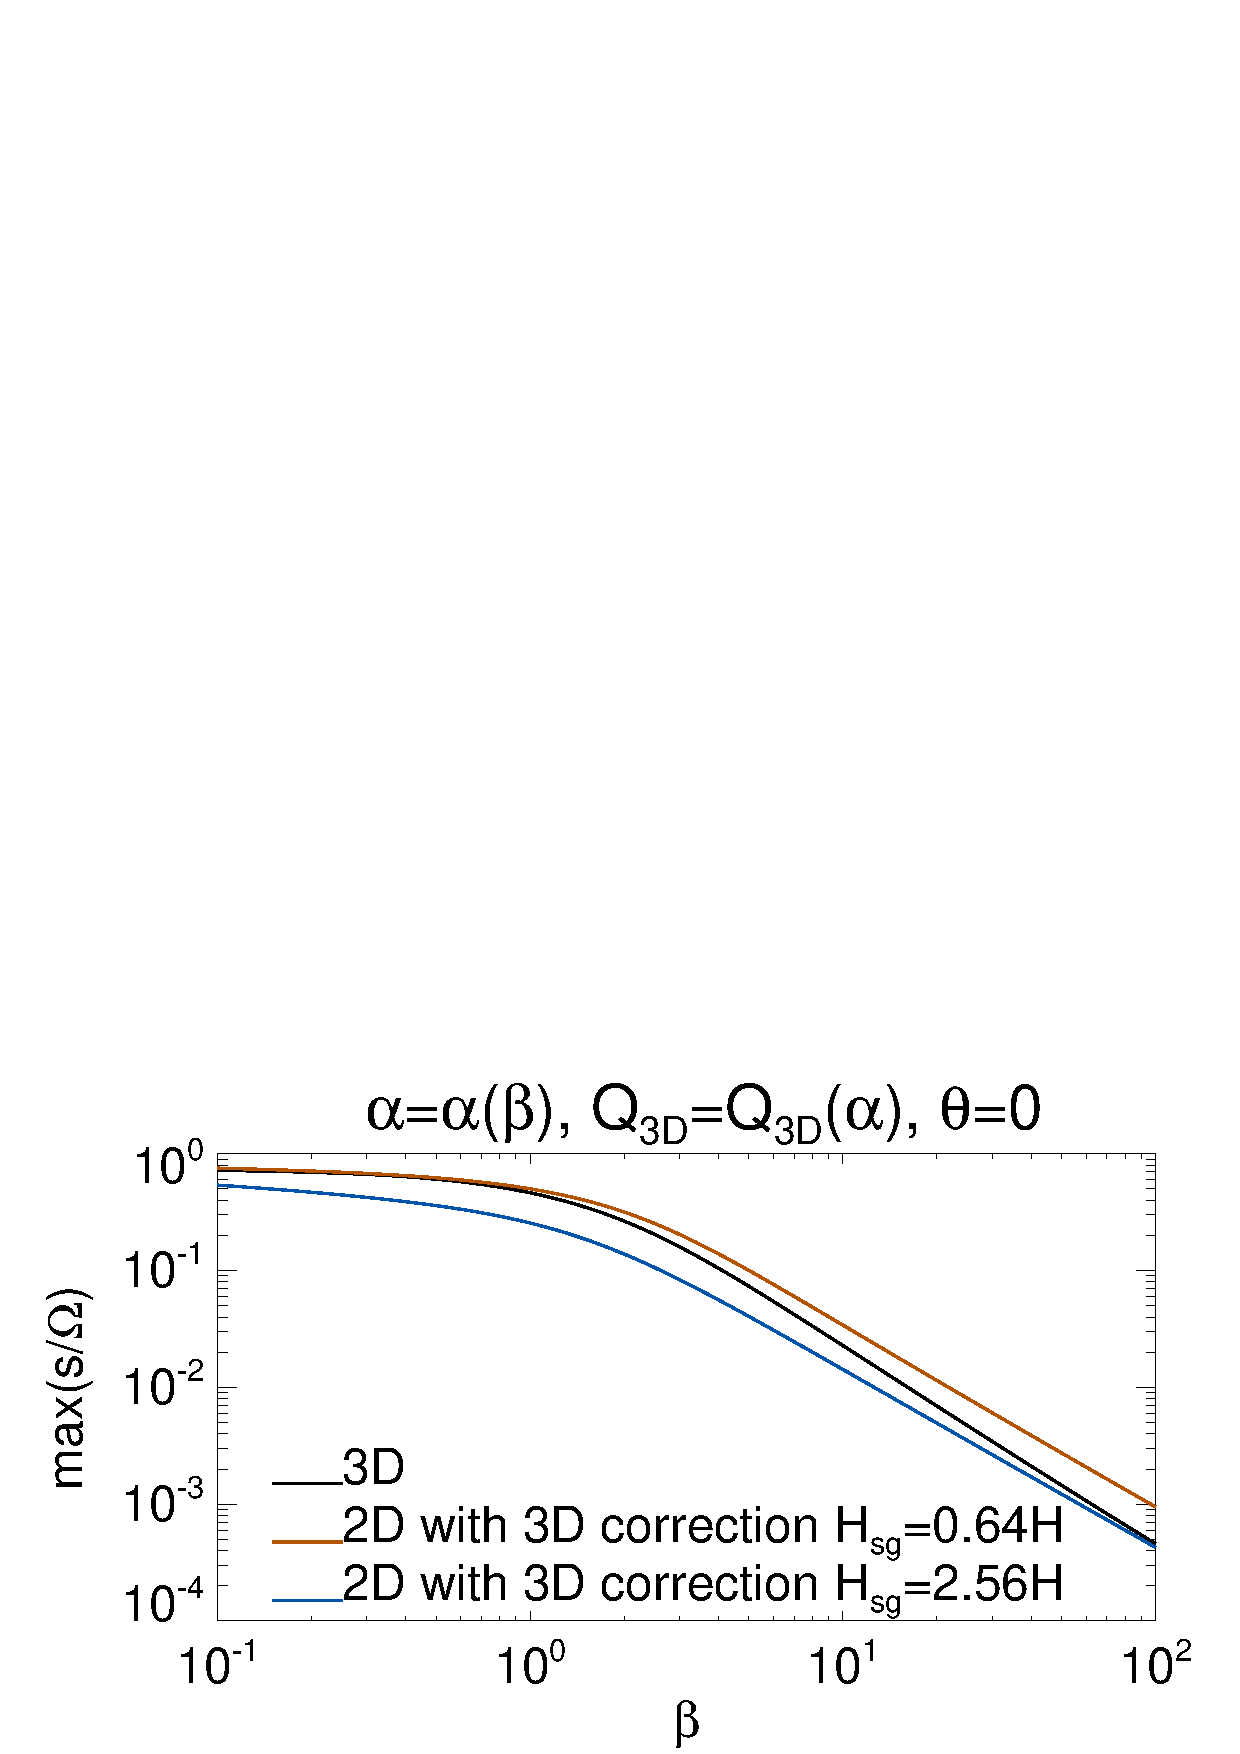
\includegraphics[width=\linewidth,clip=true,trim=0cm 0.cm 0.cm
    0.0cm]{figures/growth_visc3d}
  \caption{Growth rates from the viscous 3D eigenvalue problem (black solid
    line). Asterisks and diamonds are obtained from the 2D dispersion
    relation (Eq. \ref{thindisk}) with softened gravity as described
    in Appendix \ref{3dcorr}. \label{3d_visc}} 
\end{figure}



\begin{figure}
  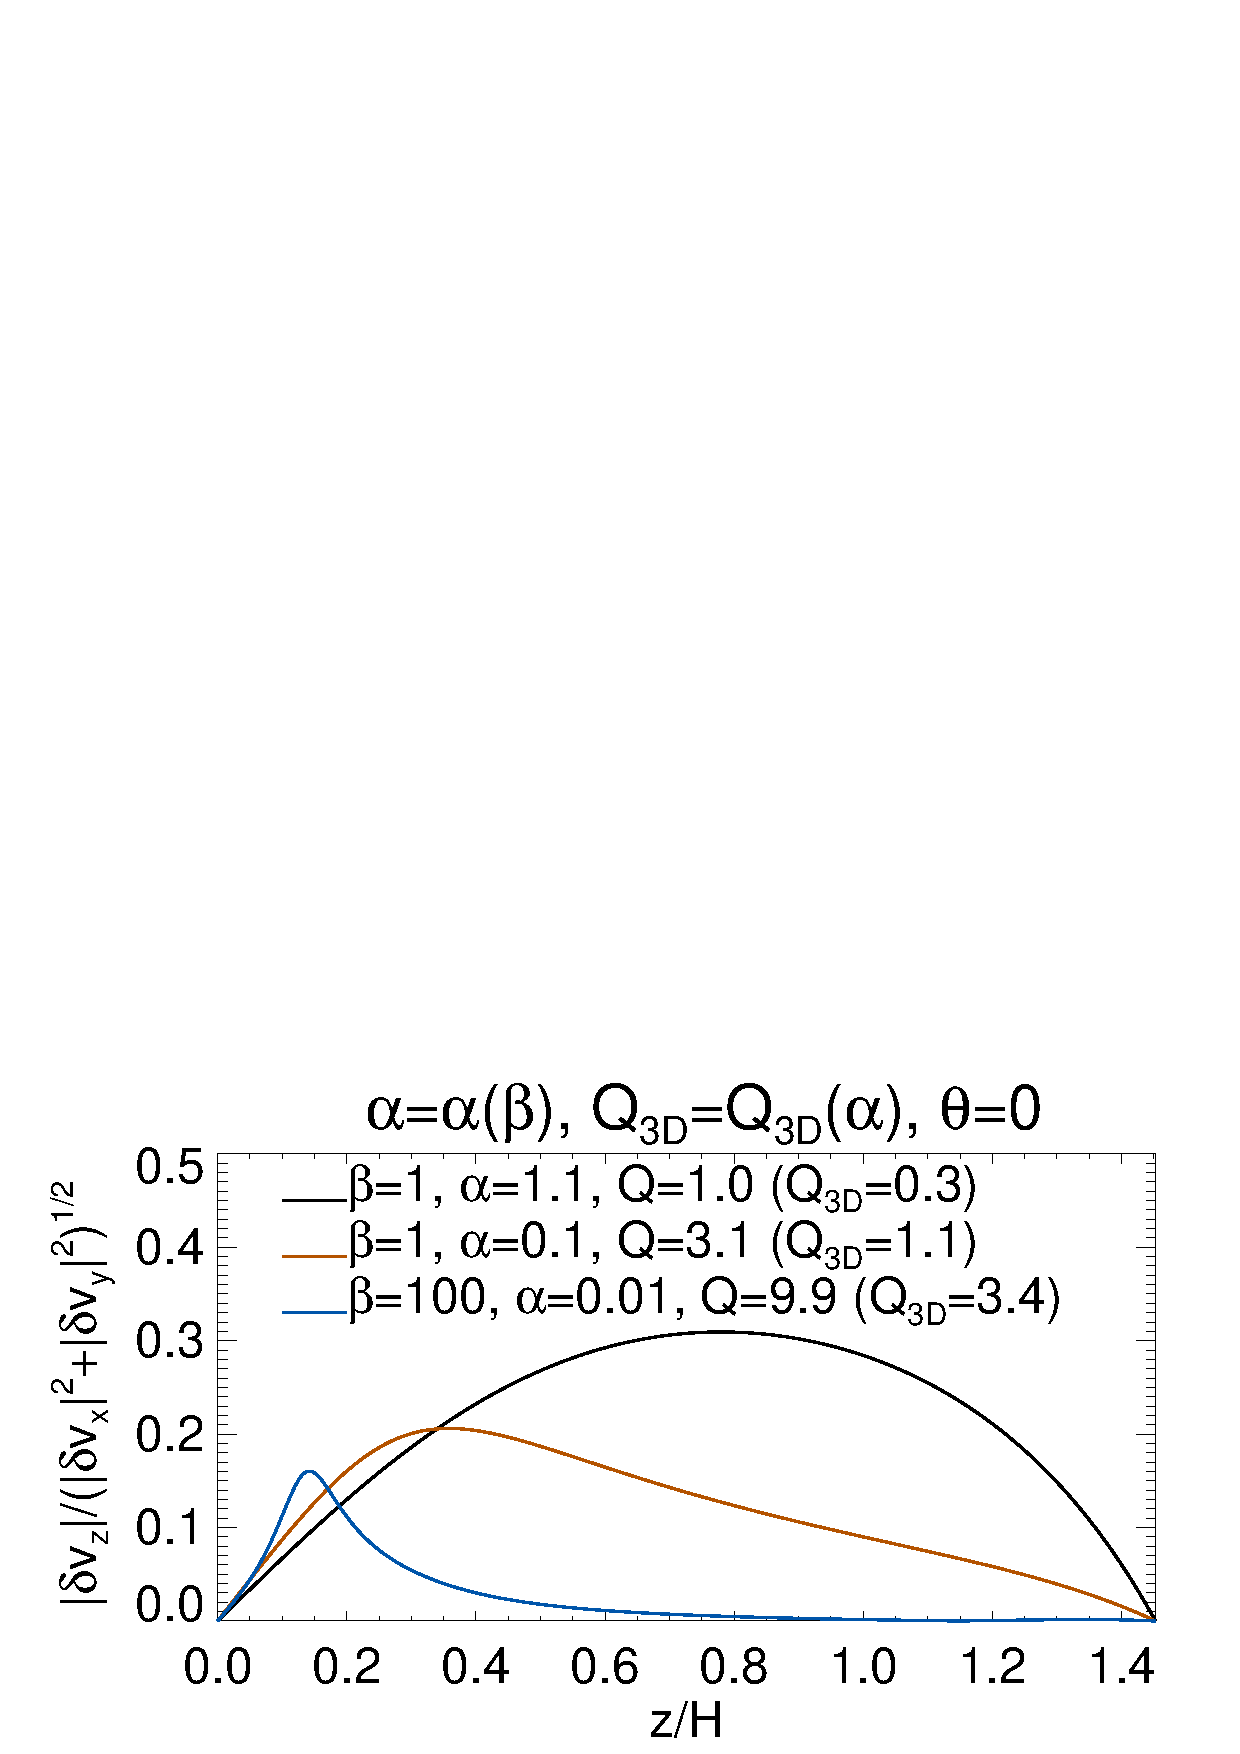
\includegraphics[width=\linewidth,clip=true,trim=0cm 0.cm 0.cm
    0.0cm]{figures/eigenvec_vz}
  \caption{Magnitude of vertical velocities, normalized by the
    magnitude of the total horizontal velocity, of the viscous GI in 
    Fig. \ref{3d_visc}, for three cooling times: $\beta=1,\,10$, and $100$. \label{3d_visc_vz}} 
\end{figure}
